% ----------------------------------------------------------
% Parte de revisão de literatura
% ----------------------------------------------------------
\section{Introduction}

%  Is my research question clear?
%
%  Does my Introduction act as a clear road map for understanding my paper?
%
%  Is it sufficiently different from the Abstract, without any cut and pastes? (\hl{some} overlap is fine)
%
%  Have I mentioned only what my readers specifically need to know and what I will subsequently refer to in the Discussion?
%
%  Have I been as concise as possible?
%
%  Have I used tenses correctly? present simple (general background context, description of what will be done in the paper), present perfect (past to present solutions), past simple (my contribution, though this may also be expressed using the present simple or future simple)

% It explains why there is a need or a problem and how the author will deal with it. The introduction usually motivates the present study, provides a literature review, and explains how the current work fits with what has gone before.

%    1    What is the problem?
%    2    Why is it interesting and important?
%    3    Why is it hard? (E.g., why do naive approaches fail?)
%    4    Why has not it been solved before? (Or, what's wrong with previous proposed solutions? How does mine differ?)
%    5    What are the key components of my approach and results? Also include any specific limitations.
One of the most costly operations involving software development is maintenance, it has been reported that above 75\% of the total software cost is used for maintenance activities~\citep{bennett2000software, liu2012schedule}. A important factor regarding it is the quality of the written code, since it affects the readability of the code, and hence its maintainability~\citep{aggarwal2002integrated}, since software maintainers spend around 60\% of their time understanding the code they are working at~\citep{abran1993measurement}. But even in cautiously designed systems, the quality of the source code tends to degrade as the project evolves, since a system’s original design is rarely prepared for every new requirement and the quick changes made by different people without properly adjusting the system’s structure~\citep{seng2006search}. Another factor is that developers also tends to focus on the addition of the new functions and bug fixes rather than improving software maintainability~\citep{tufano2015and}.  They also tend to overlook it when it is seemly complex and when it seems not to be critical to maintain the longevity of the software~\citep{murphy2012we}

A common way to avoid this degradation is to identify and fix those flaws as they appear. In object oriented code, one of the main descriptions of these code issues are the code smells~\citep{mens2004survey}. Code smells provide heuristics for the identification of design flaws in the source code that make software harder to evolve, comprehend and maintain. Each code smell examines a specific kind of system elements (class, methods, etc...) that can be evaluated by its characteristics~\citep{olbrich2009evolution}. For example a commonly occurring code smell is the duplicated code, where you have codes with the same behaviour in different parts of the application as follows:
\begin{lstlisting}
public interface Employee {
    double calculate_salary();
}
public class Director implements Employee {    
    public double calculate_salary() {  //duplicated code
        return self.dailyPayment * self.workedDays;
    };
}
public class Manager implements FileType {
    public double calculate_salary() { //duplicated code
        return self.dailyPayment * self.workedDays;
    };
}
\end{lstlisting}

In the snippet possible to notice that the \textit{calculate\_salary} method has the same implementation among the different \textit{classes}, this code is problematic since as the code-base grows since if you change the code in one of the classes and do not change it in another you can introduce an inconsistent behaviour in your application, leading to an increase in the software complexity and stacking of bad quality code. Another example of code smells is the Data Class, this smell indicates classes that only have fields and properties but no behaviour, as shown on the code snippet:

\begin{lstlisting}
public class Employee{    
    public string name;
    public string address;
    public Date birth_date;
    public double salary;
}
\end{lstlisting}

This kind of class hurt the object orientation principles by having a class without any behaviour, but in many cases and architectures, such as for \textit{ViewModels} in MVC architectures this is a desirable behaviour. In those scenarios it would not be considered a code smell by the developers but an architectural option. As shown on the previous scenario the code smells provides many guidelines to identify unwanted behaviour and common coding mistakes, but it is still dependent on the programmers interpretation~\citep{fowler1999refactoring}, since it can have different interpretations according to the scenario. The definition of what is and what is not a code smell in a given context may not be a consensus among developers working in the same application~\citep{bryton2009strengthening, fontana2016comparing}. Making their identification an error-prone and time-consuming task given the size of some commercial applications~\citep{murphy2012we}.

In order to reduce this subjective interpretation, automated approaches based on the source code were presented in previous works~\citep{fontana2012automatic, fokaefs2007jdeodorant, mantyla2004bad, rasool2015review}, but a relevant part of those approaches are based on code metrics.~\citep{bryton2010reducing, counsell2010strategy, marinescu2004detection, moha2010decor, rasool2015review}. These techniques uses metrics and thresholds that are not consistent among them, leading to an increasing number of false positives, not representing real problem~\citep{fontana2016comparing}. Since it does not consider information related to the context, domain, size and design of the system~\citep{ferme2013real}. In this scenario, Machine Learning techniques can be used to capture this subjectivity. Machine learning techniques are used for a wide range of applications such as risk management~\citep{cowell2007modeling}, medicine~\citep{akay2009support}, biology~\citep{kell2006metabolomics}, financial markets~\citep{doostmohammadi2017day} among others~\citep{fenton2007managing, li2017deep}. And can also be used for the identification of code smells in source code, providing further flexibility in comparison to the current metrics based approaches~\citep{kotsiantis2007supervised}.

This study has as primary objective the identification of which methods and practices are mostly used when applying machine learning for code smells identification and which machine learning techniques are being applied for code smells identification. For that end we developed a mapping study on Machine Learning techniques and code smells found in literature, covering papers from the introduction of anti-patterns in 1999 by~\cite{fowler1999refactoring} up to and including papers publishing until December 2016.  The design flaws were categorized under the definition of the works defined by~\cite{fowler1999refactoring} and~\cite{brown1998antipatterns}. The study resulted in the classification of 26 papers out of 53 researched papers, separated and categorized by design flaws and applied techniques, we found that regarding f-measure the best average performance was provided by Decision Tree, followed by Random Forest, Semi-supervised and Support Vector Machine Classifier techniques. While Bayesian Network, Linear Discriminant Analysis and Naive Bayes presented the worst performance overall between the studied practices. 

This chapter was organized according to the following structure:  Section 2 provides a background research about code smells, refactoring, and Machine Learning techniques; Section 3 presents the related works; Section 4 addresses the methodology used for this work; Section 5 displays the results of the SLR; Finally, Section 6 discusses the results of the work and provides suggestions for future work.


\section{Background}

\subsection{Code smells}

There has been extensive researches focusing on the study of bad design practices, also called code smells, defects, anti-patterns or anomalies~\citep{sahin2014code}. But code smells is widely used to address source code level flaws. This concept was firstly introduced by~\citet{fowler1999refactoring} and was initially defined as "indications that there is trouble that can be solved by refactorings". They represent "poor" solutions to recurring implementations and design problems that impede the maintenance and evolution of programs~\citep{khomh2011}. Code smells are symptoms, which can, but not necessarily have to, point to an actual issue. Therefore, they are not patterns to be avoided, but easy to notice signals that require a more thorough examination~\citep{walter2016relationship}.  Follows a short description of each smell proposed by~\citet{fowler1999refactoring}:
\begin{itemize}
	\item \textbf{Long Method (LM)} is a method that is long, so it is hard to understand, change or extend.
	\item \textbf{Large Class (LC)} is a class that tries to do a load of things, having plenty of instance variables or methods.
	\item \textbf{Primitive Obsession (PO)} represents the usage of primitives instead of small classes, making it less meaningful and reusable.
	\item \textbf{Long Parameter List} is a parameter that is very long and difficult to represent.
	\item \textbf{Data Clumps (DAC)} data items that usually appear together.
	\item \textbf{Switch Statements (SS)} usage of type codes or run-time class type detection instead of polymorphism.
	\item \textbf{Temporary Field (TF)} the class has a variable which is only used in specific situations.
	\item \textbf{Refused Bequest (RB)} a child class does fully support its parent implementation.
	\item \textbf{Alternative Classes with Different Interfaces (ACDI)} a case where a class can operate with alternative classes but the interface of these classes is different.
	\item \textbf{Parallel Inheritance Hierarchies (PIH)} a situation where two parallel class hierarchies exists but are related.
	\item \textbf{Lazy class (LAZ)} a class that is not doing enough and should be removed.
	\item \textbf{Data class (DC)} a class that contains data but does not contain logic.
	\item \textbf{Duplicate Code (DUC)} a code that does the same thing as another piece of code.
	\item \textbf{Speculative Generality (SG)} when unnecessary code is created anticipating future changes on software.
	\item \textbf{Message Chains (MC)} a chain of calls from one object to another, without adding any new behaviour.
	\item \textbf{Middle Man (MM)} when a class delegates a great deal of its behaviour to another class.
	\item \textbf{Feature Envy (FE)} a method that is more interested in other classes properties then its the ones from its own class.
	\item \textbf{Inappropriate Intimacy (II)} when two classes are tightly coupled.
	\item \textbf{Divergent Change (DC)} when a class need to be changed every-time another class is changed.
	\item \textbf{Shotgun Surgery (SS)} when a class changes requires a broadcast changing of other classes.
	\item \textbf{Incomplete Library Class (ILC)} When the software uses an incomplete library.
	\item \textbf{Comments (COM)} misuse of comments to compensate poor code structure.
\end{itemize}

~\citet{mantyla2003bad} categorized code smells into 8 categories: 
\begin{itemize}
    \item \textbf{The Bloaters:} Represents something that has grown so large that it cannot be effectively handled. This category cover the following smells: Long-Method; Large Class; Primitive Obsession; Long Parameter List; and Data Clumps.
    \item \textbf{The Object-Orientation Abusers:} Represents code that do not exploit the possibilities of Object-Oriented Design (OOD). The following smells are included in this category: Switch Statements; Temporary Fields; Refused Bequest; Alternative Classes with Different Interfaces; Parallel Inheritance Hierarchies.
    \item \textbf{The Change Preventers:} Smells that prevent or hinder the changing or further development of the system. This category is composed by: Shotgun Surgery and Divergent Change.
    \item \textbf{The Dispensables:} Represent something that is unnecessary and should be removed from the code. Represented by the smells: Lazy class; Data class; Duplicated Code and Speculative Generality.
    \item \textbf{The Encapsulators:} Smells that deals with data communication or encapsulation, including Message Chains and Middle Man.
    \item \textbf{The Couplers:} Smells that increases the coupling of the system, being composed by Feature Envy and Inappropriate Intimacy
    \item \textbf{Others:} Smells that do not fit in any of the previous categories and are not comparable, such as: Incomplete Library Classes and Comments.
\end{itemize}

Code smells can also be considered as symptom of a design level flaw, also known as anti-patterns~\citep{moha2010decor}. The anti-patterns concept was introduced by~\citet{brown1998antipatterns} putting it as a literary form that describes a recurrent solution to a problem that generates decidedly negative consequences. The studies also use approaches to identify the code anti-patterns instead of code smells, since they describe more generic flaws, in this study we use three of them:
\begin{itemize}
	\item \textbf{The Blob}: corresponds to a large controller class that depends on data stored in surrounded data classes. A large class declares fields and methods with a low cohesion. A controller class monopolizes  the processing done by a system, takes the main decisions, and directs the processing of other classes. 
    \item \textbf{The Functional Decomposition}: consists of a main class  in which inheritance and polymorphism are scarcely used, associated with small classes, which declare a great deal of private fields and implement only sparse methods.
    \item \textbf{The Spaghetti Code}: classes with no structure, declaring long methods with no parameters, and utilizing global variables for processing. Names of classes and methods may suggest procedural programming.
\end{itemize}

The main purpose to identify design flaws is to fix it before it degrades, this practice of improving the design of an existing piece of code without of changing its behavior is known as refactoring~\citep{granhem2014model}. Refactoring aims to restructure the internal structure of object-oriented software without changing its external behaviors, to improve the quality of software~\citep{fowler1999refactoring}. It is a safe and effective technique to improve the quality of software because it guarantees preserving the observable behavior of software. In addition, refactoring has been widely accepted as an important activity in software development and maintenance~\citep{lee2011automated}. 

\subsubsection{Code smell identification}


Code smell identification techniques can be classified in 7 categories according to their nature, as categorized by~\citet{rasool2015review}:
\begin{enumerate}
    \item \textbf{Manual code smell detection techniques:} Manual techniques presented by researchers when Fowler identified code smells
    \item \textbf{Metrics-based techniques:} Similar in concepts to the manual techniques as they depend on source code metrics, but they differ in how they apply metrics and which types of code smells they focus on.
    \item \textbf{Symptoms-based techniques:} Use different symptoms/notations translated into detection algorithms. The conversion of symptoms into detection rules requires analysis and interpretation effort to select proper threshold values
    \item \textbf{Visualization-based code smell detection techniques:} Use the semi-automated process for the detection of code smells. These techniques integrate the capability of human expertise with the automated detection process. The limitation of these techniques is human effort, and they have scalability problems for large systems. These techniques are also error prone because of wrong human judgment.
    \item \textbf{Probabilistic-based code smell detection techniques:} Apply bayesian and fuzzy logic rules that include quantitative properties and relationships among classes. These techniques rank candidate smells using fuzzy logic inference rules and handle uncertainty in the code smell detection process
    \item \textbf{Search-based code smell detection techniques:} Apply different algorithms for the detection of code smells directly from source code. Usually, the techniques in this category apply machine learning algorithms. These techniques learn from standard design and coding practices and examine how code deviates from these practices
    \item \textbf{Cooperative-based code smell techniques:} Perform different activities in a cooperative way for improving performance of activities. The cooperative-based techniques became more common in the later years, as they can improve accuracy and performance for code smell detection
\end{enumerate}

From the techniques above, the manual one is the best known, it eliminates uncertainties of the process, but due to its human-centric approach it is time-consuming and error prone~\citep{counsell2010strategy}. The techniques 2 and 3 uses thresholds to determine the presence or absence of code smells, but its accuracy is dependent on the proper selection of threshold values, which are usually empirical and unreliable~\citep{ferme2013real}. The forth approach tries to reduce the uncertainty with the use of both human and automated approaches. While the remaining ones use statistical or machine learning approaches to try to reduce this uncertainty but require large amounts of human annotated data and it also dependant on the quality of this data~\citep{rasool2015review}.

\subsubsection{Empirical studies on code smells}
Empirical researches demonstrated a relationship between structural attributes (design metrics) and external quality metrics (code smell and class error tendencies)~\citep{shatnawi2008effectiveness}. Another study found that the process of smell detection can serve as a systematic method for identifying and restructuring problematic classes. In the same study, it was also examined the presence of six code smells, finding that the Shotgun Surgery smell showed correlation with increased defect proneness~\citep{li2007empirical}. The result was questioned afterward in an analysis of 7 open source systems: that found no correlation between Feature Envy and Shotgun Surgery with high defect proneness~\citep{dambros2010impact}. 

A further experiment showed that only a handful of the issues could be interpreted with smells, while problems such as Appropriate Naming, Architecture and Existing defects could not be captured with the smell analysis~\citep{yamashita2012code}. A study by~\cite{hall2014some} examined the relation between defects and five code smells. Results were again inconclusive: some code smells appeared to have no effect on the defect-proneness (e.g. Switch Statements), others increased it (e.g. Message Chains), other reduced the number of defects (e. g.  Middle Man and Speculated Generality), and the results for other smells (e. g. Data Clumps) were inconclusive. The study by \citet{palomba2014reallysmell} investigates the developers perceptions regarding the code smells and found that the following smells are not perceived as design problem: Class Data Should Be Private, Middle Man, Long Parameter List, Lazy Class, and Inappropriate Intimacy. They also may or may not represent the “intensity” of the problem and that smells related to complex/long source code are perceived as a threat. An experimental study concerning the impact of dependencies between classes with design patterns and anti patterns on defect and change proneness demonstrated that classes having dependencies with anti-patterns exhibit more defects than those with dependencies with design patterns~\citep{jaafar2016evaluating}. Another study also found that code smells do have a negative impact on classes~\citep{khomh2009exploratory}

These works demonstrated that the impact of code smells in the quality of the code varies, depending on the individual smell, and on the analyzed system~\citep{walter2016relationship}. Another important factor is that the manual recognition of code smells on the source depends on the developer’s degree of experience and perception, which is error prone and time-consuming~\citep{counsell2010strategy}, since part of the time the developers are not aware of their presence in the code~\citep{yamashita2013developers}.

\subsection{Machine Learning} 

Machine learning algorithms instances can be represented using the same set of features. The features may be continuous, categorical or binary~\citep{kotsiantis2007supervised}. Machine learning techniques can be mainly categorized in three ways: supervised, unsupervised and semi-supervised. If instances are given with known labels (the human annotated correct output) then the learning is called supervised, otherwise, when the instances are unlabeled it is unsupervised learning~\citep{jain1999data}. There is also a hybrid approach, which is the semi-supervised learning that uses both labeled and unlabeled data to perform an otherwise supervised learning or unsupervised learning task~\citep{zhu2011semi}.

Numerous Machine Learning applications involve tasks that can be set up as supervised~\citep{kotsiantis2007supervised}, which is also the leading approach used for code smells identification~\citep{fernandes2016review}. The major supervised approaches were identified by~\citet{kotsiantis2007supervised} in his literature review, as follows:
\begin{itemize}
    \item \textbf{Decision Trees:} Decision trees are trees that classify instances by sorting them based on feature values. Each node in a decision tree represents a feature in an instance to be classified, and each branch represents a value that the node can assume. Instances are classified starting at the root node and sorted based on their feature values. 
    \item \textbf{Learning Set of Rules:} Decision trees can be translated into a set of rules by creating a separate rule for each path from the root to a leaf in the tree. However, rules can also be induced from training data using a variety of rule-based algorithms.
    \item \textbf{Single layered perceptrons:} Uses a single layer of weights to define a linearly separable binary classification.
    \item \textbf{Multi layered perceptrons (Artificial Neural Network):} Created to solve non linear classification problems that cannot be solved by a single layer. A multi-layer neural network consists of large number of units (neurons) joined together in a pattern of connections. 
    \item \textbf{Radial Basis Function (RBF) network:} An RBF network is a three-layer feedback network, in which each hidden unit implements a radial activation function and each output unit implements a weighted sum of hidden units outputs.
    \item \textbf{Naive Bayes:} Naive Bayesian networks (NB) are simple Bayesian networks which are composed of graphs with only one unobserved node and a chain of children observed nodes, with a assumption of state independence between child nodes and their parent. The Naive Bayes is based on estimating the probabilities of the unobserved node, based on the observed ones.
    \item \textbf{Bayesian networks:} A Bayesian Network (BN) is a graph based model that establishes a probability relationships among a set of known variables. The Bayesian network structure is a graph containing nodes linked with its features. The features must be conditionally independent from their non-descendants in relation to its parents.
    \item \textbf{Instance Based learning:}  Instance-based learning algorithms is a statistical based and lazy-learning algorithms, as they delay the induction or generalization process until classification is performed
    \item \textbf{Support Vector Machines (SVM):} SVMs re based on the notion of a “margin” in either side of a hyperplane separating two features. Its optimizing objective is to increase the margin and create the largest distance between features in the hyperplane. The complexity is unaffected by the number of features. So SVMs are suited to deal with learning tasks where the number of features is large with respect to the number of training instances.
\end{itemize}

Unsupervised learning are composed mainly by Clustering Techniques. The clustering objective is to develop an automatic algorithm that discovers the natural groupings in the unlabeled data~\citep{jain1999data}. Clustering algorithms can be broadly divided into two groups: hierarchical and partitional. Hierarchical clustering algorithms recursively find nested clusters, while the partitional clustering find the clusters simultaneously. In semi-supervised clustering, instead of specifying the class labels, constraints are specified, as a weaker way of encoding the labeled data. Semi-supervised learning can be applied in place supervised learning, using unlabeled data for training~\citep{jain2010data}. Semi-supervised learning has been applied to natural language processing (word sense disambiguation , document categorization, named entity classification, sentiment analysis, machine translation), computer vision (object recognition, image segmentation), bio-informatics (protein function prediction), and cognitive psychology~\citep{zhu2011semi}.

Machine learning techniques has also been used to address code smell identification problems, as exposed by Figure \ref{fig:smellDetectionTechniquesRelation}.

\begin{figure}[hbt] 
	\caption{Code smell techniques relationship}
	\label{fig:smellDetectionTechniquesRelation}
	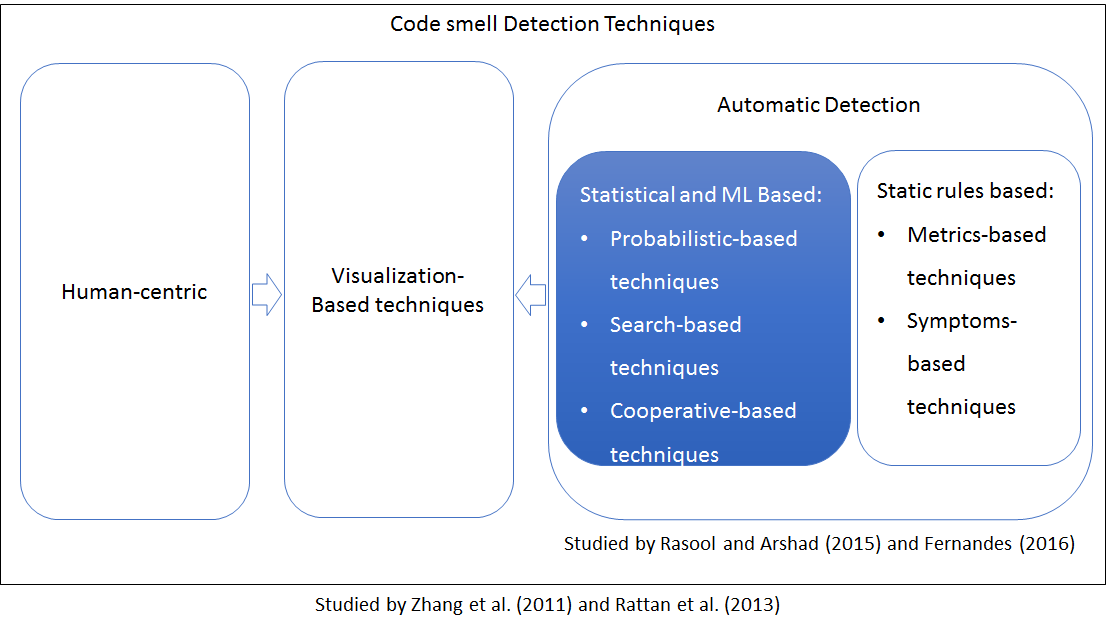
\includegraphics[width=0.95\textwidth]{imagens/smellDetectionTechniquesRelation.png}
\end{figure}

\section{Related work}

The following studies regards reviews of code smell identification.~\citet{zhang2011code} reviewed 39 papers, searching for studies about any of the code smells, to assess how they contribute to the understanding of these code smells and their impact in the system maintainability, that study focuses in manual and static based techniques since Machine Learning based techniques were rare at the moment when the study happened, while our study focus only on Machine Learning techniques for code smell identification.

The study by~\citet{rattan2013software} reviewed 213 studies regarding software clone identification, finding a lack definition of what a clone is and also a lack of empirical research regarding the harmfulness of clones. This study is different from ours since it focus in only one code smell and also do not focus on any particular technique or study type.

\citet{al2015identifying} performed a review on 47 studies about the identification of opportunities for code refactoring activities. It tried to find what kind of refactoring techniques were more common and which techniques were used to identify these refactorings opportunities and how they were evaluated. Regarding this last objective it has found a lack of standardized and empirical data to support the techniques. This study differs from ours since it focus on refactoring rather than code smell.

A review by~\citet{rasool2015review} covered 46 papers on the techniques and tools used for mining code smells from the source code of different software, it evaluates and compares the coverage of the smells by the techniques and their performance, it found out that the techniques are dependent on the proper selection of threshold values. This study has a broader scope than ours, trying to compare all the code smells and techniques, not focusing on the Machine Learning techniques and by doing so it does not analyze the used techniques, their nature and performance.

The~\citet{fernandes2016review} review covered 107 papers regarding code smell detection tools, identifying a high redundancy between the smells identified by the tools, showing the need of better comparisons to choose appropriate tools for each smell. Our study differs from this, given that it focuses only on tools, but does not give a clue on the algorithms or techniques used by those tools.

\section{Research Method}

%   How can I assess the quality of my Methods section? To make a self-assessment of your Methods section, you can ask yourself the following questions.
%    * Have I really described my Methods in a way that is easy for readers to follow and which would enable them to replicate my work? Have I ensured that I have covered every step? Is my structure clear and complete?
%    * Have I been as concise as possible? Have I used references to previous works rather than repeating descriptions that readers could easily find elsewhere?
%    * Do the individual sentences in each paragraph contain too many, too few, or just the right manageable number of steps? Have I ensured that my sentences don’t sound like lists?
%    * Have I thought about the way readers prefer to receive information? (no ambiguity, no back referencing, everything in chronological order, headings, bullets)?
%    * Have I checked my grammar (infinitive, gerund, allow, thus etc.) with regard to how I outline how and why I made certain choices?
%    * Have I checked my journal’s guidelines on how to use numbers?
%    * Have I used tenses correctly? past simple (in the passive form to describe what I did), present simple (descriptions of established scientific fact)

This study performed a mapping study about the usage of Machine Learning techniques for code smells identification. SLRs are reviews organized and based on a clear search strategy, that ensures the rigor, completeness and reproducibility of the process, focusing on the identification, evaluation and interpretation of the available research that is relevant to a particular question~\citep{kitchenham2010systematic}.

In order to accomplish the SLR the following steps were taken: planning, defining research questions, searching databases, discussion of validity, data extraction, and synthesis of the results, those steps are in accordance to the typical steps taken for a SLR~\citep{keele2007guidelines}. The following subsections embrace each of those steps.

\subsection{Planning}

We developed a review protocol in order to ensure that the research is executed in a planned way and not driven by the researcher expectations according to the guidelines provided by Kitchenham et al.~\cite{kitchenham2015evidence}. In the protocol, the following items were addressed as part of the planning for the study: research objectives; research questions; search strategy; study selection, studies quality assessment; data extraction; and data synthesis and aggregation.

\subsection{Research Questions}

 This research focuses on the identification machine learning techniques for code smells identification and in order to accomplish that the following questions must be addressed: 

\begin{itemize}
    \item \textbf{RQ1: Which code smells are addressed by articles using machine learning techniques for code smells identification?}
    RQ1 focuses on the most studied code smells covered by the literature. It can help identify which code smells have not been explored in existing research and can be used as gaps for future works.
    \item \textbf{RQ2: Which machine learning techniques are used when identifying code smells?} 
    RQ2 aims in the identification of machine learning techniques  commonly used to identify code smells and it can list potential machine learning techniques that were not yet explored for this specific task.
    \item \textbf{RQ3: Which machine learning techniques are most used for each kind of code smell?}
    RQ3 is concerned with the relationship between the machine learning techniques and the code smells in research papers allowing the identification of which techniques are used for each of the code smells. It could also lead us to identify potential machine learning techniques that can be used for similar code smells but have not yet being used with this intent.
    \item \textbf{RQ4: Which machine learning techniques performs better for each code smell?}
    RQ4 compares the performance of different machine learning techniques for code smell detection. The answer to this question can help researchers define which machine learning techniques to use when studying different types of code smells.
\end{itemize}

\subsection{Search Strategy}

In order to find relevant articles to achieve the goals of this study, we conducted searches based on the recommendations by Kitchenham et al.~\cite{kitchenham2015evidence}. In the first step, we used personal experience to define the list of journals and conferences, summarized in table~\ref{tab:ManualSearchSources}, used to establish the quasi-gold standard. The digital libraries selected for automated searches were ACM, IEEE, Science Direct and Wiley.

was used in manual searches by two of the authors authors and 69 articles resulted of the .
in four digital libraries - ACM, IEEE, Science Direct and Wiley - for papers published up to 2016. The definition of the search string followed these steps based :
\begin{enumerate}
    \item{Derived major terms for machine learning and code smells from research questions.}
    \item{Broke major terms down into smaller terms.}
    \item{Identified alternative spellings or synonyms for the smaller terms.}
    \item{Checked the search terms in known relevant papers.}
    \item{Used Boolean operator OR to combine alternative spellings and synonyms. Used Boolean operator AND to link machine learning and code smells terms.}
\end{enumerate}

The following search string was then generated: "("code smell" OR "bad smell") AND ("learning" OR "data mining" OR "artificial intelligence" OR "pattern recognition" OR "case based reasoning" OR "decision tree" OR "regression tree" OR "classification tree" OR "neural net" OR "genetic programming" OR "genetic algorithm" OR "Bayesian belief network" OR "Bayesian net" OR "association rule" OR "support vector machine" OR "support vector regression")". 

This filter returned 1021 papers, distributed as shown in Figure \ref{fig:librariesImage}. The search string tries to filter papers that applies Machine Learning techniques for code smell identification problems.

\begin{figure}[hbt] 
	\caption{Distribution of papers by article}
	\label{fig:librariesImage}
	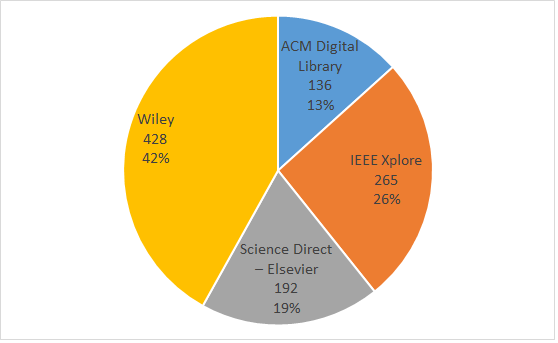
\includegraphics[width=0.95\textwidth]{imagens/librariesDistributionImage.png}
\end{figure}

After the filtering, 338 duplicated results were removed, resulting in 683 remaining results. Following to that publications which were not papers or proceedings papers which belonged to a Journal that is not related to Computational Fields were removed and, leaving 286 results left. The studies were then filtered by the publication title, removing any study which was not related to the usage of Machine Learning techniques for code smells identification, what left 155 results. This same criteria was applied when filtering by abstract, resulting in 53 papers left for classification. These steps were summarized in Figure \ref{fig:paperScreening}  Each step was peer reviewed by graduated students, the  results were compared and discussed to reach a consensus.

\begin{figure}[hbt] 
    \centering
    \caption{Paper screening process}
	\label{fig:paperScreening}
	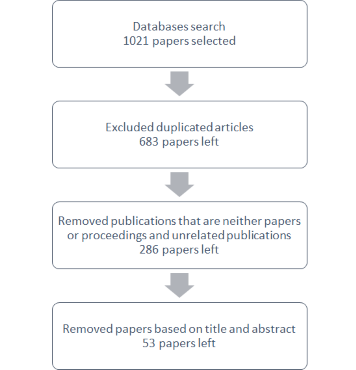
\includegraphics[]{imagens/paperScreening.png}
\end{figure}

The inclusion and exclusion criteria for those filters were defined as follows:

\noindent \textbf{Inclusion criteria:}
\begin{itemize}
    \item Articles describing the use of methods and that establish the relationship between machine learning and code smells.
    \item The studies publication type must be journals or conferences
\end{itemize}

\noindent \textbf{Exclusion criteria:}
\begin{itemize}
    \item Remove duplicates
    \item Remove studies where the code smells identification are done manually
    \item Remove non-empirical studies
\end{itemize}

\subsection{Quality assessment}

The main purpose of this study is to cover papers about the usage of Machine Learning Techniques for Code Smell identification. In order to try to avoid the non inclusion of relevant papers  precautions were taken. One of the cautions made was to include keywords, title, and abstract in the search, we also took the precaution of including synonyms and abbreviates.

Clear criteria for the exclusion and exclusion of the papers were also defined prior to the study. And each steps was registered so it could be evaluated by external parties. To assert the results of the study, peer reviews done by two graduated researchers were executed, compared and discussed in order to reach a consensus and avoid the perception of the researcher to influence the results. Criteria for classification was also selected from related works and explicit defined before the execution of the review.

The following questions were taken to improve the reliability of the work and avoid missing relevant papers:
\begin{itemize}
    \item \textbf{QA1}: Are the aims of the research defined explicitly?
    \item \textbf{QA2}: Is the context related to code smells?
    \item \textbf{QA3}: Are the used techniques exposed and related to Machine Learning?
    \item \textbf{QA4}: Is the experimental design appropriate and justifiable?
    \item \textbf{QA5}: Is the proposed estimation method comparable with other methods?
    \item \textbf{QA6}: Are the findings of study stated and supported by reporting results?
    \item \textbf{QA7}: Does the study add value to academia or industry community?
\end{itemize}

\section{Results}

%How can I assess the quality of my Results section? To make a self-assessment of your Results section, you can ask yourself the following questions.
%    * Have I expressed myself as clear as possible, so the contribution of my results give stands out for the referees and readers?
%    * Have I limited myself to only reporting the key result or trends each figure and table conveys, rather than reiterating each value?
%    * Have I avoided drawing conclusions? (this is only tr,ue when the Results is an independent section)
%    * Have I chosen the best format to present my data (e.g. figure or table)? Have I ensured there is no redundancy between the figures and tables?
%    * Have I ensured my tables of results are comprehensive in the sense that they do not exclusively include points wich prove my point?
%    * Have I mentioned only what my readers specifically need to know and what I will subsequently refer to in the Discussion?
%    * Have I mentioned any parts of my methodology (e.g. selection and sampling procedures) wich could have affected my results?
%    * Have I used tenses correctly? past simple for your findings (in the passive form), present simply (descriptions of established scientific fact)


In this section, the results of Mapping are presented, firstly, we show an overview of the selected papers and after the answers to research questions and their findings.

\subsection{Overview}

In this study we identified 26 papers that used Machine Learning techniques for code smell identification. They were published between 1999 to 2016 and they used experimentation as methodology. 65\% of the papers were published in conferences and the other 37\% were published in journal. Only 5 of publications were represented by more than one publication venue: Annual Conference on Genetic and Evolutionary Computation; International Conference on Software Engineering;Journal of Systems and Software; Expert Systems with Applications; Journal of Software: Evolution and Process. These publications represented almost half of the selected papers as shown in Table \ref{tab:papersByPublication}.

\begin{table}[hbt]
\centering
\caption{Papers by publication}
\label{tab:papersByPublication}
\begin{tabular}{ll}
\hline
Publication &                                               \# of studies\\ \hline
Annual Conference on Genetic and Evolutionary Computation &     3   \\
International Conference on Software Engineering &              3   \\
Journal of Systems and Software &                               3   \\
Expert Systems with Applications &                              2   \\
Journal of Software: Evolution and Process &                    2   \\
Others &                                                        13  \\ \hline
\end{tabular}
\end{table}

Through the Figure \ref{fig:papersByYear}  it's possible to see the trend of publication years. The Figure \ref{fig:papersByYear} shows a small interest of studies to identify code smell using Machine Learning techniques between 2002 at 2014, but big interest in 2015 at 2016. The number of research in last two years overcame the numbers of previous years.  Worth remember that code smell term were used by Kent Beck in the late 1990's and the research about code smell were focused in other techniques as metrics. Detection of code smells based in machine learning techniques have not been largely explored~\citep{Fontana2013}.
%arranjar uma justificativa melhor
%Não achei a observação nesses artigos  - Bruno
%Confirming the observation of previous studies~\citep{rasool2015review, fontana2016comparing} which shows a growing interest in Machine Learning techniques for code smell identification.
% Do Rasool se não me engano me baseei na Table II, mas do Fontana eu também não achei, posso ter interpretado algo errado ou mudado algo no caminho quando estava escrevendo

\begin{figure}[hbt] 
    \centering
	\caption{Papers by year}
	\label{fig:papersByYear}
	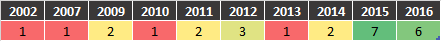
\includegraphics[]{imagens/papersByYear.png}
\end{figure}
%todos os papers usaram java? -Bruno
%23 ou 24 projetos de código fonte aberto
%os outros projetos que são 70% não nomearam os sistemas? % os dados do slr_protocol_results mostram mais de 65 projetos
All papers selected in this study identified code smells analyzing projects developed with Java language. From 26 papers, 23 used open source projects, while only 3 used private data source. We identified 88 open source projects as dataset used in research, the dataset more used was the Xerces, followed by JHotDraw, Eclipse Core and ArgoUML. Among the 88 datasets 62 of them were used only one time. As detailed by Table \ref{tab:opensourceTable}.

\begin{longtable}{||c|c||c||c|}
\caption{Used open source projects}
\label{tab:opensourceTable}
\\

\hline
	Software & Number of Papers & Software & Number of Papers \\ \hline
	Xerces & 6 & Apache Commons Logging & 1 \\ \hline
	JHotDraw & 5 & JDI-Ford & 1 \\ \hline
	Eclipse Core & 5 & Apache Derby & 1 \\ \hline
	ArgoUML & 4 & JFreeChart  & 1 \\ \hline
	JFreeChart & 3 & Apache James Mime4j & 1 \\ \hline
	GanttProject & 3 & JRDF & 1 \\ \hline
	Apache Cassandra & 2 & Apache Tomcat & 1 \\ \hline
	Rhino & 2 & Maven & 1 \\ \hline
	Qualitas Corpus & 2 & ApacheAnt & 1 \\ \hline
	GanttProject  & 2 & Pixelitor & 1 \\ \hline
	jEdit & 1 & ApacheAnt  & 1 \\ \hline
	Ant & 1 & sapphire & 1 \\ \hline
	Log4J  & 1 & Android API (framework-opt-telephony) & 1 \\ \hline
	And Engine & 1 & XWorks & 1 \\ \hline
	JabRef & 1 & BCEL & 1 \\ \hline
	Apache Commons Codec & 1 & Jboss & 1 \\ \hline
	Android API (tool-base) & 1 & Closure Compiler & 1 \\ \hline
	Apache Commons IO & 1 & JDK  & 1 \\ \hline
	nebula.widgets.nattable & 1 & dltk.core & 1 \\ \hline
	Apache Commons Lang & 1 & Android API (sdk) & 1 \\ \hline
	Xerces  & 1 & Android API (frameworks-base) & 1 \\ \hline
	JGraphx & 1 & Aardvark & 1 \\ \hline
	egit & 1 & platform.resources & 1 \\ \hline
	JHotDraw  & 1 & Gitblit & 1 \\ \hline
	FindBugs & 1 & Ant-Apache & 1 \\ \hline
	jUnit & 1 & Google Guava & 1 \\ \hline
	FreeMind  & 1 & ANTLR & 1 \\ \hline
	Lucene  & 1 & graphiti & 1 \\ \hline
	GanttAzureus & 1 & Xom & 1 \\ \hline
	Mongo DB & 1 & Guava & 1 \\ \hline
	Android API (frameworks-support) & 1 & Apache Ant & 1 \\ \hline
	Nutch  & 1 & Hibernate & 1 \\ \hline

\end{longtable}


\subsection{Which code smells are addressed when using Machine Learning techniques for the identification?}

In this study, we used the 22 code smells defined by~\cite{fowler1999refactoring} as base for our classification, we also used 3 of the anti-patterns defined by~\citep{brown1998antipatterns} related to code related design flaws. There is also the "others" classification meant to capture smells defined by other authors and code-flaws not related to a specific smell, since the authors aim at code metrics optimization instead of a specific smell.

%código duplicado ficou em outra classificação? - Bruno Zhang citou que código duplicado é mais estudo nos code smells. Mas a o mapeamento não mostrou isso
Comparing the studied code-related design flaws using machine learning, the ones with higher appearance were Feature Envy (FE) smell and BLOBs both studied by 5 papers, followed by Long Methods (LM) that appeared in 4. While Comments (COM), Primitive Obsession (PO), Refused Bequest, Alternative Classes with Different Interfaces (ACDI) and Incomplete Library Class (ILC) were not addressed by any of the studied papers. The distribution of the smells is show in Figure \ref{fig:papersBySmell}. Except for the duplicated code which is usually the mainly studied smell, the other smells are coherent with the ones identified by~\cite{zhang2011code} in his review. The others category, composed mainly by optimization in the code metrics appeared 8 times, using alternatives to the traditional code smells. %O que nós fizemos com estes outros?

\begin{figure}[!ht] 
    \centering
	\caption{Papers by Code Smell}
	\label{fig:papersBySmell}
	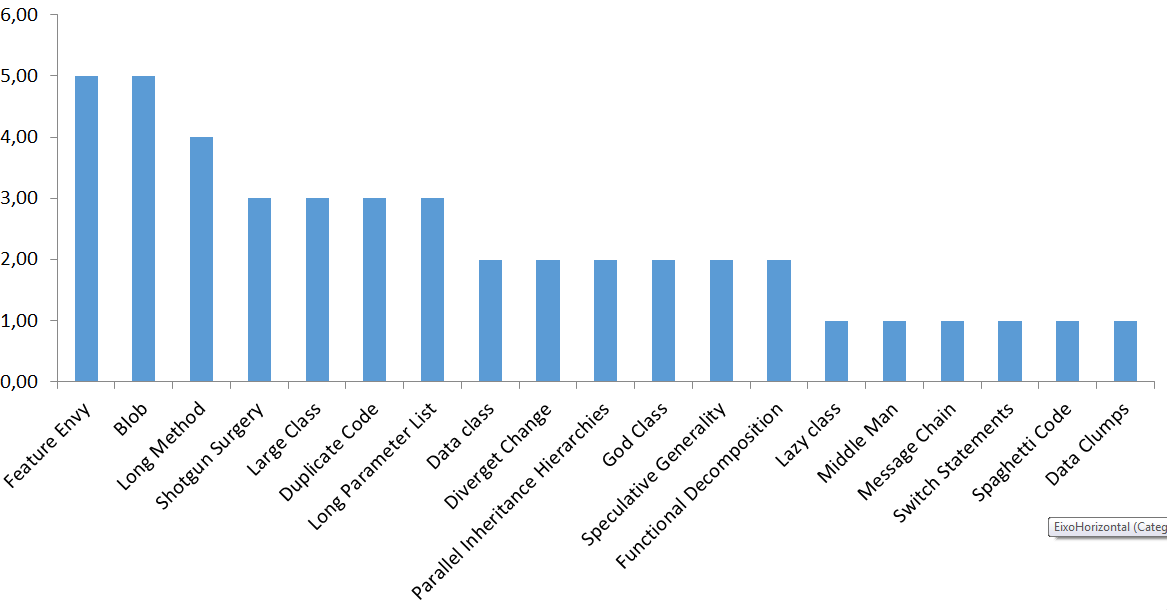
\includegraphics[width=0.95\textwidth]{imagens/papersBySmell.png}
\end{figure}

% Montar um gráfico que abrange as classificações dos tipos e dos bad smells - Decidir entre o o gráfico ou a frase abaixo. 
% Gerar um insight para falar do gráfico - Bruno
When grouping by the classification defined by~\cite{mantyla2003bad} it is possible to observe that the main focus regarding the addressed type of smell are the Bloaters representing 35\% of the studied smells. Follows to this: The Dispensables (15\%); The Object-Orientation Abusers (9\%); The Change Preventers (9\%); The Couplers (9\%); The Encapsulators (4\%). The other code smells, mainly represented by metrics-based representations, represent 17\%. As detailed on Figure \ref{fig:papersBySmellType}.

%alterar o gráfico para deixar mais nítido.

\begin{figure}[!ht] 
    \centering
	\caption{Papers by Code Smell Type}
	\label{fig:papersBySmellType}
	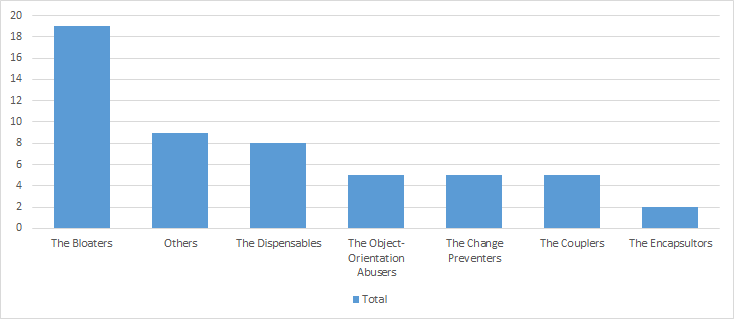
\includegraphics[width=0.95\textwidth]{imagens/papersBySmellType.png}
\end{figure}

%
%%There are a strongest co-ocorrece of code smells in studies. For instance, the research between...
% Não entedi porque eles são relacionados só pq foram definidos or brown? - Bruno
When studying the smells usually studied together, one of the strongest co-occurrence is between BLOB, Spaghetti Code (SC) and Functional Decomposition (FD), one of the main reasons is that they use the anti-patterns definition  by~\citet{brown1998antipatterns}, while the others are defined by ~\citet{fowler1999refactoring}. Duplicated code also had a strong co-occurrence with Divergent Changes (DCP) and Shotgun Surgery (SS), but the reciprocal was not true, one of the explanations is that Duplicated Code (DUC) is usually studied alone. Feature Envy also receives highlight when comparing smells usually studied together, it is studied together with part of the smells. Others that deserve mention are Long Parameter List (LPL), Long Methods (LM) and Large Class (LC). The co-occurrence matrix is shown in details in Figure \ref{fig:smellsCoOccurrence}.  %essa figura não disse o q está descrito no texto. Talvez um gráfo represente bem essa relação. Podemos tentar gerar no gephi mesmo

\begin{figure}[!ht] 
    \centering
	\caption{Graph representing which smells worked in the same paper}
	\label{fig:smellsCoOccurrence}
	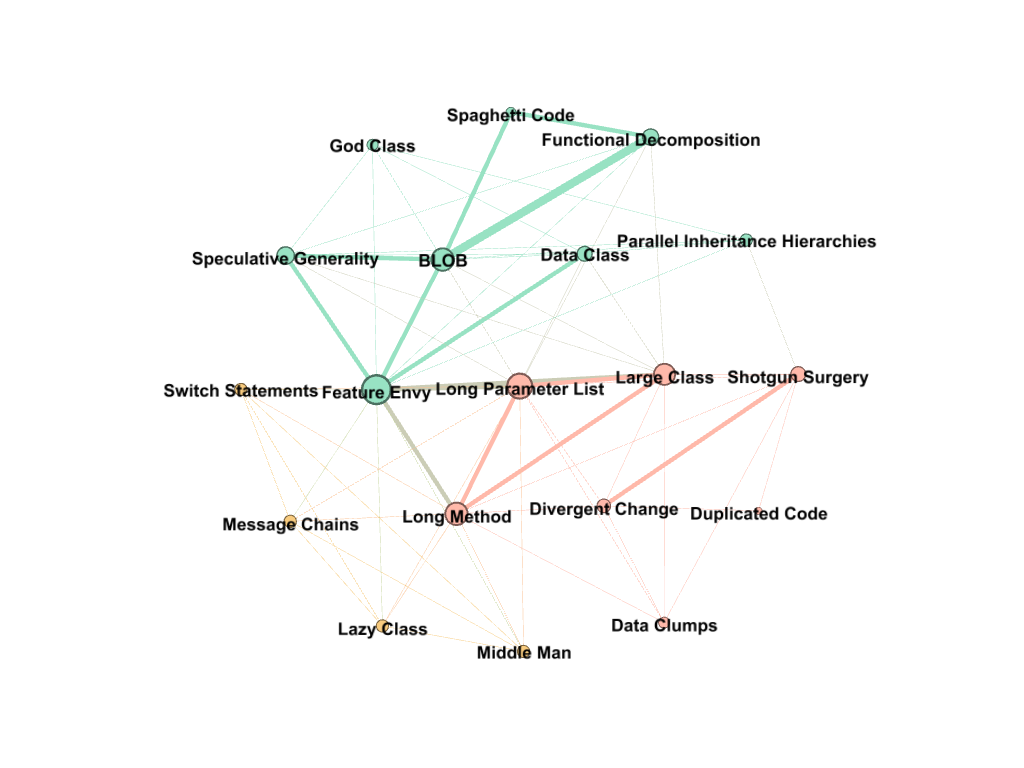
\includegraphics[width=0.95\textwidth]{imagens/smells_coocurrence_graph.png}
\end{figure}


\subsection{Which Machine Learning techniques are used when identifying code smells?}

The leading technique in the analyzed papers was the Genetic Algorithm which appeared 8 times, this technique is used mainly in search-based techniques, and focuses on optimizing one or more metric by mutating and evolving the code. Followed by Naive Bayes Classifiers that appeared 4 times. While a approaches such as: Linear discriminant analysis (LDA); Decision Tree; Support; Vector Machine (SVM); Directed Acyclic Graph (DAG); Text-Based - appeared only once. The distribution can be visualized in Figure \ref{fig:papersByMLTechnique}.

\begin{figure}[!ht] 
    \centering
	\caption{Papers by Machine Learning Technique}
	\label{fig:papersByMLTechnique}
	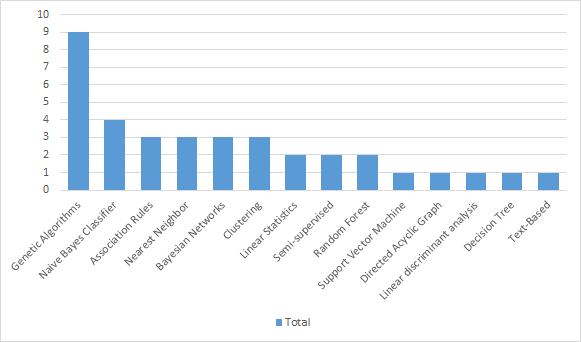
\includegraphics[width=0.95\textwidth]{imagens/papersByMLTechnique.png}
\end{figure}


Regarding the kind of technique used the supervised techniques were the main one, being used in 32 tests (88\%); Semi supervised and unsupervised techniques appeared only 2 (6\%) times which. The results was expected since supervised tests are the greatly used in researches~\citep{kotsiantis2007supervised}.

\subsection{Which Machine Learning techniques are most used for each kind of code smell?}

The smells addressed by the techniques were coherent with the smells that appeared in the related papers, showing a high level of redundancy. The smell focused by the majority of the techniques was Feature Envy (FE), which was aimed by 9 techniques (64\%). Followed by Long Method (LM) with 8 techniques (57\%) and Long Parameter List (LPL) with 7 (50\%). From the smells targeted by the studied papers, the ones covered by less techniques were Speculative Generality (SG), Spaghetti Code (SC), Data Class (DAC),  God Class (GC), Parallel Inheritance (PIH) and Divergent Changes (DCP) with 2 techniques each (14\%).

From a Machine Learning technique perspective, the Association Rules techniques was the technique with broader usage, covering 13 smells (59\% of them), followed by linear statistics with 11 smells (50\%), Naive Bayes and Random Forest with 9 smells (43\%). While Text-Based and Linear Discriminant Analysis with 1 smell (5\%) are in the lower half.


When comparing the number of times a code smell was addressed by a given technique, there was no clear relationship. Although the smells coverage is higher for a given technique, e. g., Feature Envy (FE) and Bayesian Network, it does not displays a clear pattern. The relation between smells and techniques can be visualized in Figure \ref{fig:smellsXMLTechniques}

\begin{figure}[!ht] 
    \centering
	\caption{Number of times a smell was studied with another by technique}
	\label{fig:smellsXMLTechniques}
	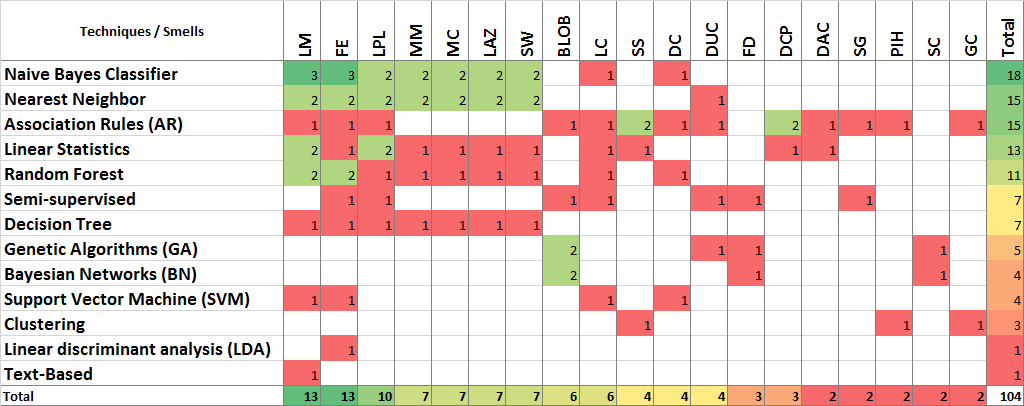
\includegraphics[width=0.95\textwidth]{imagens/smellsXMLTechniques.png}
\end{figure}

However when comparing the smells by type, we found out that the Association Rules technique with a relevant focus on the Change Preventers type of smell, as the graph nature of technique allows it to analyze the relationship between methods and classes. The other smell types followed the same patterns presented when comparing the coverage by papers and the classifiers the same pattern as discussed previously.

\begin{figure}[!ht] 
    \centering
	\caption{Code Smell type by Machine Learning technique}
	\label{fig:smellsTypeXMLTechniques}
	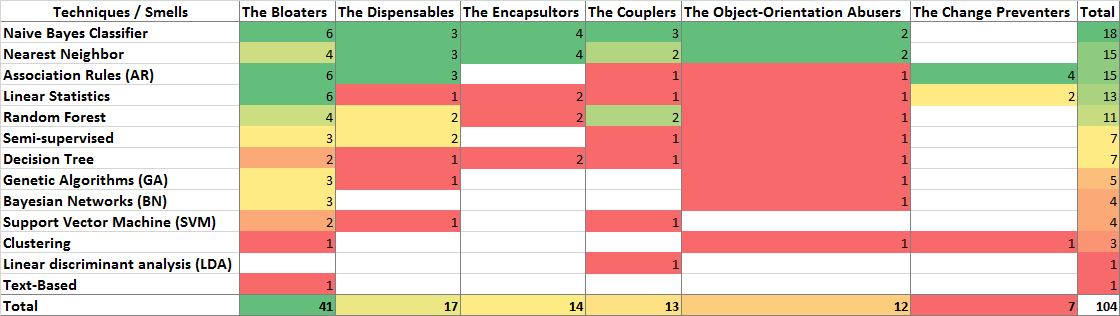
\includegraphics[width=0.95\textwidth]{imagens/smellsTypeXMLTechniques.png}
\end{figure}

\subsection{Which Machine Learning techniques performs better for each smell?}

One hardship we found when comparing the techniques performance is the lack of standardized data. 14 out of the 26 papers provided performance info. From those, 13 provided precision data, 12 provided recall values and only 6 provided us with F-measures, we used the recall and precision data provided by the other to calculate their f-measures as well to have a better comparison measure. To have comparable parameters we also selected only the papers that used the same baseline as the majority of the articles, in this case a manual annotation of the code smells.

In terms of f-measure the best average performance was provided by Decision Tree, followed by Random Forest, Semi-supervised and Nearest Neighbor techniques. While Text-Based, Linear Discriminant Analysis and Naive Bayes presented the worst performance overall between the studied practices, as demonstrated by Figure \ref{fig:fmeasureByTechniques}.

\begin{small}
\begin{longtable} {|l|l|l|l|l|}
\caption{F-Measure summary per smell and technique: Ordered by the max f-measure}
\label{tab:opensourceTable}
\\

\hline
Smell            & Technique                          & Min   & Median & Max    \\ \hline
MM - Middle Man              & Decision Tree          & 1.00  & 1.00   & 1.00  \\ \hline
MM - Middle Man              & Linear Statistics      & 0.85  & 0.85   & 0.85  \\ \hline
MM - Middle Man              & Nearest Neighbor       & 0.85  & 0.85   & 0.85  \\ \hline
MM - Middle Man              & Random Forest          & 0.71  & 0.71   & 0.71  \\ \hline
MM - Middle Man              & Naive Bayes Classifier & 0.14  & 0.38   & 0.62  \\ \hline\hline

SG - Speculative Generality  & Association Rules (AR) & 0.86  & 1.00   & 1.00  \\ \hline\hline

DCP - Divergent Change       & Association Rules (AR) & 0.55  & 0.85   & 1.00  \\ \hline\hline

LM - Long Method             & Association Rules (AR) & 0.99  & 0.99   & 0.99  \\ \hline
LM - Long Method             & Random Forest          & 0.86  & 0.92   & 0.99  \\ \hline
LM - Long Method             & Decision Tree          & 0.86  & 0.92   & 0.98  \\ \hline
LM - Long Method             & Support Vector Machine & 0.69  & 0.83   & 0.97  \\ \hline
LM - Long Method             & Naive Bayes Classifier & 0.54  & 0.60   & 0.93  \\ \hline
LM - Long Method             & Nearest Neighbor       & 0.89  & 0.90   & 0.90  \\ \hline
LM - Long Method             & Linear Statistics      & 0.84  & 0.84   & 0.84  \\ \hline
LM - Long Method             & Text-Based             & 0.56  & 0.62   & 0.71  \\ \hline\hline

LC - Large Class             & Random Forest          & 0.97  & 0.97   & 0.97  \\ \hline
LC - Large Class             & Association Rules (AR) & 0.97  & 0.97   & 0.97  \\ \hline
LC - Large Class             & Decision Tree          & 0.96  & 0.96   & 0.96  \\ \hline
LC - Large Class             & Naive Bayes Classifier & 0.96  & 0.96   & 0.96  \\ \hline
LC - Large Class             & Support Vector Machine & 0.73  & 0.85   & 0.96  \\ \hline\hline

LPL - Long Parameter List    & Random Forest          & 0.97  & 0.97   & 0.97  \\ \hline
LPL - Long Parameter List    & Linear Statistics      & 0.95  & 0.95   & 0.95  \\ \hline
LPL - Long Parameter List    & Nearest Neighbor       & 0.92  & 0.92   & 0.92  \\ \hline
LPL - Long Parameter List    & Decision Tree          & 0.92  & 0.92   & 0.92  \\ \hline
LPL - Long Parameter List    & Naive Bayes Classifier & 0.31  & 0.32   & 0.33  \\ \hline\hline

SS - Shotgun Surgery         & Decision Tree          & 0.97  & 0.97   & 0.97  \\ \hline
SS - Shotgun Surgery         & Nearest Neighbor       & 0.89  & 0.90   & 0.91  \\ \hline
SS - Shotgun Surgery         & Linear Statistics      & 0.89  & 0.89   & 0.89  \\ \hline
SS - Shotgun Surgery         & Random Forest          & 0.89  & 0.89   & 0.89  \\ \hline
SS - Shotgun Surgery         & Naive Bayes Classifier & 0.52  & 0.61   & 0.70  \\ \hline\hline

FE - Feature Envy            & Decision Tree          & 0.96  & 0.96   & 0.96  \\ \hline
FE - Feature Envy            & Support Vector Machine & 0.69  & 0.83   & 0.96  \\ \hline
FE - Feature Envy            & Naive Bayes Classifier & 0.24  & 0.26   & 0.95  \\ \hline
FE - Feature Envy            & Random Forest          & 0.94  & 0.94   & 0.94  \\ \hline
FE - Feature Envy            & Association Rules (AR) & 0.86  & 0.86   & 0.86  \\ \hline
FE - Feature Envy            & Nearest Neighbor       & 0.84  & 0.84   & 0.84  \\ \hline
FE - Feature Envy            & Linear Statistics      & 0.75  & 0.75   & 0.75  \\ \hline\hline

DUC - Duplicated Code        & Semi-supervised        & 0.96  & 0.96   & 0.96  \\ \hline
DUC - Duplicated Code        & Association Rules (AR) & 0.72  & 0.85   & 0.85  \\ \hline\hline

MC - Message Chains          & Linear Statistics      & 0.86  & 0.86   & 0.86  \\ \hline
MC - Message Chains          & Nearest Neighbor       & 0.86  & 0.86   & 0.86  \\ \hline
MC - Message Chains          & Random Forest          & 0.80  & 0.80   & 0.80  \\ \hline
MC - Message Chains          & Naive Bayes Classifier & 0.67  & 0.71   & 0.76  \\ \hline
MC - Message Chains          & Decision Tree          & 0.66  & 0.66   & 0.66  \\ \hline\hline

GC - God Class               & Clustering             & 0.66  & 0.72   & 0.82  \\ \hline\hline

BLOB                         & Bayesian Networks (BN) & 0.60  & 0.69   & 0.79  \\ \hline\hline
\end{longtable}

\end{small}

\begin{figure}[!ht] 
    \centering
	\caption{Machine Learning techniques F-measure Box-plot}
	\label{fig:fmeasureByTechniques}
	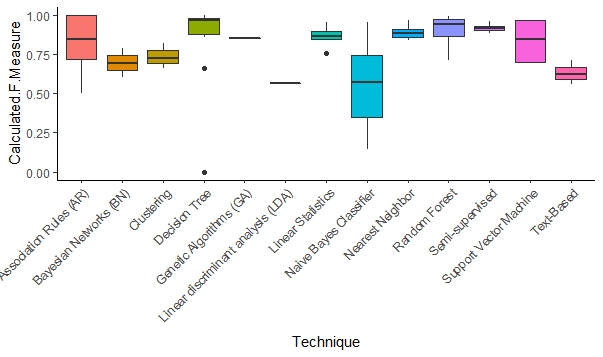
\includegraphics[width=0.9\textwidth]{imagens/fmeasureByTechniques.png}
\end{figure}

When comparing the results by f-measure as demonstrated by Figure \ref{fig:techniqueXSmellFMeasure}, it is possible to notice that the Association Rules technique performed above the others for Divergent Changes (DCP) and Speculative Generality (SG) smells, the ones covered by only this technique. But performs poorly for Duplicated Code (DUC) and Feature Envy (FE), when compared to the other techniques. Decision tree was also the best performing technique for Middle Man and Shotgun Surgery smells, while Random Forest had an outstanding performance for Long parameter list and Semi-Supervised techniques for Duplicated Code. Naive Bayes on the other side, performed poorly for Long Parameter List, Middle Man and Shotgun Surgery. In regard to the other smells, there was no outstanding technique.

\begin{figure}[!ht] 
    \centering
	\caption{Technique F-Measure by code smell}
	\label{fig:techniqueXSmellFMeasure}
	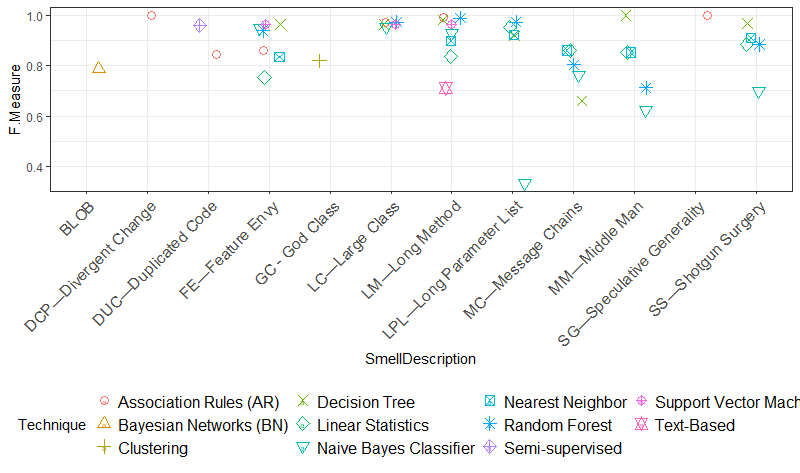
\includegraphics[width=0.95\textwidth]{imagens/TechniqueXSmellFMeasure.png}
\end{figure}

When analyzing the techniques by precision, the Linear Discriminant Analysis technique presented the best average performance, followed respectively to its performance by Association Rules, Semi-supervised and Decision Tree. In this aspect the worst performing techniques were the Bayes based techniques: Naive Bayes Classifier and Bayesian Networks. The results can be visualized in Figure \ref{fig:precisionByTechniques}.

\begin{figure}[!ht] 
    \centering
	\caption{Machine Learning techniques Precision Box-plot}
	\label{fig:precisionByTechniques}
	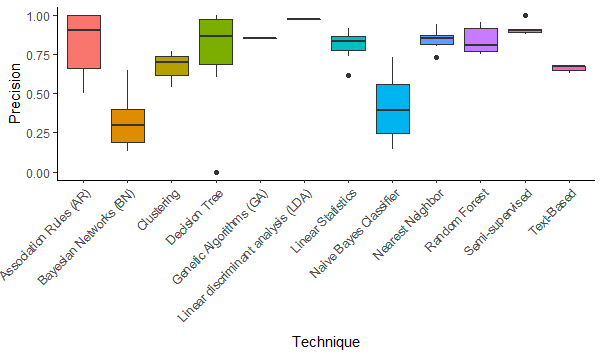
\includegraphics[width=0.9\textwidth]{imagens/precisionByTechniques.png}
\end{figure}

Comparing the techniques by precision, Association Rules, also demonstrated an outstanding performance on Divergent Changes (DCP) and Speculative Generality (SG), where it is the only technique used. Semi-supervised techniques had an outstanding performance for Duplicated Code (DUC), Random Forest for FE and Decision Tree for Lazy Class (LZC) and Middle Man (MM) also deserves mention. We had the Bayesian Networks and Naive Bayes Classifiers performing poorly than the other techniques on the smells. Those observations are displayed in Figure \ref{fig:techniqueXSmellPrecision}.

\begin{figure}[!ht] 
    \centering
	\caption{Technique Precision by code smell}
	\label{fig:techniqueXSmellPrecision}
	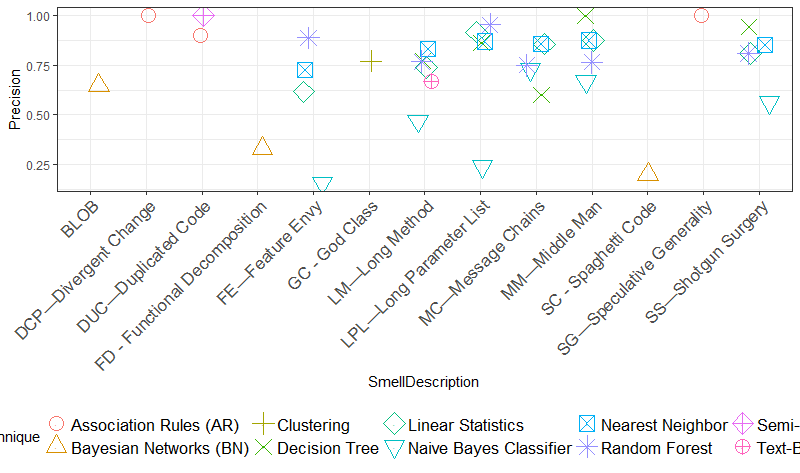
\includegraphics[width=0.95\textwidth]{imagens/TechniqueXSmellPrecision.png}
\end{figure}

When compared by recall, the techniques, in general, performed above 80\%. The best performing techniques under this perspectives were: Bayesian Networks, Decision Tree, Random Forest, Nearest Neighbor, Linear statistics, Semi-supervised, Genetic Algorithm and Clustering. While the worst performing was Naive Bayes classifier, Text-Based and Linear Discriminant Analysis, as displayed by Figure \ref{fig:recallByTechnique}.

\begin{figure}[!ht] 
    \centering
	\caption{Machine Learning techniques recall Box-plot}
	\label{fig:recallByTechnique}
	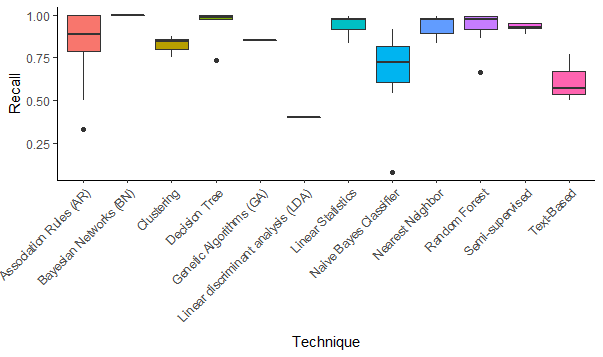
\includegraphics[width=0.9\textwidth]{imagens/recallByTechnique.png}
\end{figure}

%Calcular o F-measure de todos os papers para comparar - Bruno
Assessing the technique by smells under a Recall perspective as demonstrated in Figure \ref{fig:techniqueXSmellRecall}. As occurred in the previous perspective we have the Naive Bayes classifier performing worst in general, other techniques which displayed a bad performance was Random Forest for Middle Man (MM), Decision Tree for Message Chain (MC) and Text-Based technique for Long Method (LM).

\begin{figure}[!ht] 
    \centering
	\caption{Technique Recall by code smell}
	\label{fig:techniqueXSmellRecall}
	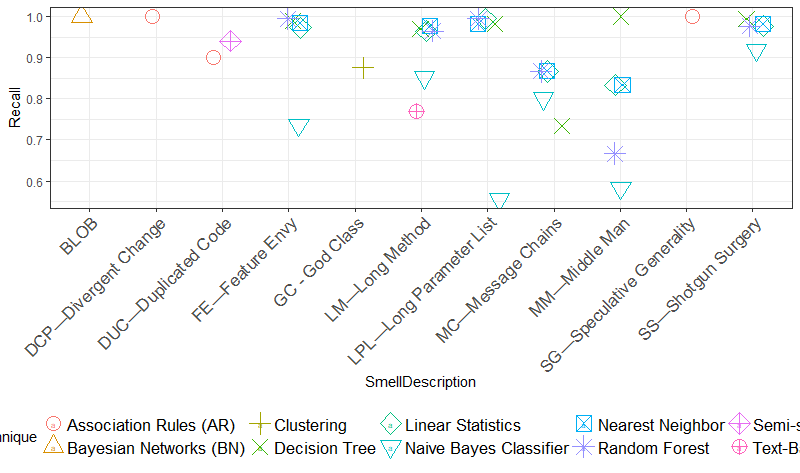
\includegraphics[width=0.95\textwidth]{imagens/TechniqueXSmellRecall.png}
\end{figure}

%as bases de dados podem ter influenciado no resultado? Seria interessante mostrar as técnicas seperadas por base dados. tipo - Usando Jhot eles procuraram os code smells x com tecnica y -Bruno

%montar uma analise de qual dataset foi utilizado para detectar qual code smell e com qual técnica de ML - Bruno
% ideia verificar o tratamento dos dados. Se ele teve que transformar os dados para um xml, csv, grafo, uml etc...
%%%%%%%%%
\section{Discussion}
\label{sec:discussion}
%%%%%%%%%

This studied tried to comprehend the patterns regarding machine learning applied for code smells identification. The study covered the papers in the period of 1999 to 2016, however no paper was published on the matter for about 2 years after the publication of the code smells by~\cite{fowler1999refactoring}, and it has only been an active topic research for the last 2 years, as shown on Table \ref{tab:papersByPublication}.

Studying the smells it was possible to assert that contrary to other studies~\citep{fowler1999refactoring, rasool2015review, fernandes2016review} that showed the Duplicated Code as the leading  smell, the ones using Machine Learning showed more concern about Feature Envy, BLOB and Long Methods, focusing heavier on non-structural smells. There is also a increasingly focus on metrics aimed technique, that seek the improvement of code metrics instead of aiming at a specific smell.

Regarding the techniques, although techniques such as Naive Bayes and Nearest Neighbor have been used more frequently than the others due to their simplicity, on the overall we did not find any killer technique receiving more attention, corroborating with the study by~\cite{fernandes2016review}, which found a high redundancy between the detected smells. The exception was the Association Rules, which outperformed the others when used for Change Preventers smells. We can also conclude, from the gathered data, the flexibility of the Machine Learning techniques, given the heterogeneous nature of the researched smells.

Comparing the performances we found that in average Decision Tree, followed by Random Forest, Semi-supervised and Nearest Neighbor classifiers outperformed the other techniques, while Text-Based, Linear Discriminant Analysis and Naive Bayes presented the worst performance overall between the studied practices, going against~\cite{fontana2016comparing} findings that found the Bayes approaches performing better for different code smells. There were also techniques that performed better for specific smells such as Association Rules for Divergent Changes and Speculative Generality, Decision tree for Lazy class, Middle Man and Shotgun Surgery smells, Random Forest for Long parameter list and Semi-Supervised techniques for Duplicated Code. 

This study also found that the papers lack comparable results, using the same data and performance metrics, a recurring problem in a significant number of studies so far~\citep{rattan2013software, al2015identifying, rasool2015review, fernandes2016review}. This factors turns the comparison of performance metrics between techniques a harder and inaccurate task, making the results less reliable and the studies harder to reproduce.


\section{Threats to validity}

We have selected the search terms according the research questions, taking into consideration the defined acceptance criteria and have used them to retrieve the relevant studies in the four electronic databases. However, relevant studies may not use the terms related to the research questions in their titles, abstracts, or keywords. We also, purposely, left out broader terms such as refactoring and anti-patterns, in order to reduce the noise during the research stage, since terms can be referred to other fields out of code smells, leading to unrelated papers.  As a result, we may have the high risk of leaving out these studies in the automatic search process. In order to mitigate this risk we have defined a selection criteria that strictly comply with the research questions to prevent the desired studies from being excluded incorrectly. In addition, the decision regarding study selection was made through double confirmation, taking separate selections by graduated researchers and a disagreements resolution for the divergent selections. However, relevant studies may have been missed. If such studies do exist, we believe that the number of them is reduced.

Another threat to validity is that the papers uses different projects to assess the results, but even the studies that uses the same project uses different annotations to train the data, decreasing the reliability of the performance comparisons. This threat is yet increased by publication bias, where the researches tend to release only positive results, avoiding the negative results, and also tend to show that their result is outperforms the others. In order to mitigate this threat we have registered the baseline that each study used, avoiding the comparison of studies developed on different projects with different baselines.

\section{Conclusions}

%    How can I assess the quality of my Conclusions? To make a self-assessment of your Conclusions, you can ask yourself the following questions.
%    * Is what I have written really a Conclusions section? (If it is more than 200–250 words, then it probably isn’t – it needs to be much shorter)
%    * If the conclusions are included in the Discussion, have I clearly signaled to the reader that I am about to discuss my conclusions (e.g. by writing In conclusion )?
%    * Have I given a maximum of one line to comments related to descriptions of procedures, methodology, interviews etc.? (Generally such comments are not needed at all, unless the primary topic of your paper is the methodology itself)
%    * Have I avoided cut and pastes from earlier sections? Do my Conclusions differ appropriately from my Abstract, Introduction and final paragraph of my Discussion?
%    * Are my Conclusions interesting and relevant?
%    * Have I given my Conclusions as much impact as possible and have I avoided any redundant expressions?
%    * Have I avoided any unqualified statements and conclusions that are not completely supported?
%    * Is my work as complete as I say it is? (i.e. I am not trying to get priority over other authors by claiming inferences that cannot really be drawn at this stage)
%    * Have I introduced new avenues of potential study or explained the potential impact of my conclusions? Have I ensured that I have only briefly described these future avenues rather than getting lost in detail?
%    * Are the possible applications I have suggested really feasible? Are my recommendations appropriate?
%    * Have I used tenses correctly? present perfect (to describe what you have done during the writing process), past simple (what you did in the lab, in the field, in your surveys etc.)

This study have reviewed 26 papers covering Machine Learning techniques for code smells identification. For each of these smells we have evaluated the studied smells, techniques and how they relate to each other and the performance of each of theses techniques for the code smells.

We found that the techniques usually perform very close to each other, but Decision Tree, Random Forest, Semi-supervised and Nearest Neighbor techniques had an better performance overall, they also tend to be heterogeneous covering smells from different types, due to this fact, the techniques tend to have a high redundancy, without specializing in a single smell. Exceptions for those findings were the Bayes approaches that performed worst than the others, in general. The Association Rules and Decision tree algorithms displayed better usage for smells that involves the relationship between different methods, classes and structures.

We also faced problems regarding the lack of comparability of the studies, since the studies usually uses annotations done by their own personal instead of using a common base, they also did not publish the results using the same metrics, making it harder to compare and asses their performance, reducing the reliability of the study and performance assertions. In order to improve the quality of the studies and allow the growth of Machine Learning techniques for code smell, more empirical studies in a common data-set is recommended.